\documentclass[10pt]{article}
\usepackage[utf8]{inputenc}

\usepackage{fullpage}
\usepackage{amsmath,amssymb, amsfonts,amsthm}
\usepackage{mathbbol}
\usepackage{graphicx}

% these are compressed lists to help fit into a 1 page limit
\newenvironment{enumerate*}%
  {\vspace{-2ex} \begin{enumerate} %
     \setlength{\itemsep}{-1ex} \setlength{\parsep}{0pt}}%
  {\end{enumerate}}
 
\newenvironment{itemize*}%
  {\vspace{-2ex} \begin{itemize} %
     \setlength{\itemsep}{-1ex} \setlength{\parsep}{0pt}}%
  {\end{itemize}}
 
\newenvironment{description*}%
  {\vspace{-2ex} \begin{description} %
     \setlength{\itemsep}{-1ex} \setlength{\parsep}{0pt}}%
  {\end{description}}
  
\title{Stat 221 Problem Set 2}
\author{Albert Young and Marco Gentili}
\date{7 October 2014}

\begin{document}

\maketitle

\section{Task 1}
\subsection{}
We want to find the posterior distribution $P(\mu, \sigma^2, \log \vec{\theta})$. Using Bayes' rule:

\begin{equation}
\begin{split}
    P(\mu, \sigma^2, \log \vec{\theta}) &\propto P( \log \vec{\theta} | \mu, \sigma^2 ) P( \mu, \sigma^2 )\\
    &\propto \prod_{j=1}^J N(\mu, \sigma^2) \dfrac{1}{\sigma^2}\\
    &\propto \dfrac{1}{\sigma^{J+2}}\prod_{j=1}^J e^{-\frac{(x_j-\mu)^2}{2\sigma^2}}
    \end{split}
\end{equation}
where $x_j = \log\theta_j$.\\

We know that
\begin{equation}
\log \theta_j \propto N(\mu, \sigma^2)
\end{equation}
Therefore
\begin{equation}
\theta_j \propto e^{N( \mu, \sigma^2 )}
\end{equation}
 Writing out the conditional posterior for $\log \theta_j$:
\begin{equation}
\begin{split}
    P(\log \theta_j | Y, \vec{w}, \mu, \sigma^2 )&=    P( Y | \log \theta_j, \vec{w}, \mu, \sigma^2 ) P( \log \theta_j | \mu, \sigma^2 )\\
    &\propto \dfrac{1}{\sigma^3}
    e^{-\frac{(x_j-\mu)^2}{2\sigma^2}} \prod_{i = 1}^N \dfrac{e^{-w_je^{x_j}}(w_je^{x_j})^{Y_{ji}}}{Y_{ji}!}
\end{split}
\end{equation}

The first term of the product comes from $P(\log \theta_j | \mu, \sigma^2)$. The second term of the product comes from the product of the Poisson probabilities of the $N$ observed values.\\

Taking the $\log$ of this, and eliminating all terms that don't have a dependence on $x_j$ (since we're just looking for the form of the answer with respect to $x_j$) we get:
\[\log P(\log \theta_j | Y, \vec{w}, \mu, \sigma^2 ) = -(x_j-\mu)^2 + \sum_{i=1}^N -w_je^{x_j} + Y_{ji}x_j\]
The second derivative of this with respect to $x_j$ is clearly always negative, so the conditional posterior is log-concave.


\section{Task 6}
To generate the graphs, we decided (for convenience) to generate 12 different $\log\vec{\theta}$, which were used to generate 50 data sets $Y_1\ldots Y_{50}$; this procedure produced 600 simulations. We chose 50 simulations per node, which would easily be completed in under an hour when testing on our local machine. However, due to demand on Odyssey the simulations took slightly longer to run.

For each of the graphs in the following sections, coverage1 refers to the first set of given parameter values, coverage2 refers to the second set, and so forth. Additionally, we bucketed the $x$-axis values by 0.1 (so if $\log(\theta_1) = 0.01$ and $\log(\theta_2) = 0.05$, they would both be under the $0$ bucket). We did this so that we would have more stability in our scatter plot estimates (i.e. points wouldn't be all over the place).
\subsection{Task 3 Discussion}
Refer to Figure 1. Naturally, the 95 percent posterior intervals exhibit higher coverage probability than the 68 percent posterior intervals (as they are wider and overlap with more values of $\log\theta_j$. In all plots, coverage probability increases with $\log\theta_j$ up to some value, after which the coverage probability plateaus. Interestingly, the coverage probability decreases after a peak at \approx $\log\theta_j = 1$ for the first set of parameters and reaches its peak at a higher value of $\log\theta_j$ for the third and fourth sets of parameters. Also surprisingly, no matter which set of parameters, the coverage probabilities appear to peak at the same level for higher values of theta, at around $0.7$ for the 68 percent interval and 95 percent for the 95 percent interval. Finally, coverage probability is consistently high for the fourth set of parameters, perhaps reflecting the greater variance to mean ratio.

\subsection{Task 4 Discussion}
Refer to Figures 2 and 3. The coverage probability with respect to $\log \theta$ is largely constant. This should be the case since each value of $w$ corresponds to many different values of $\theta$. The model $Pois(w_i\theta_i)$ has variance $w_i\theta_i$; larger values of $\log\theta_j$ correspond to greater variances and hence larger credible intervals, improving coverage. The larger spread of coverage for lower values of $log w$. Interestingly, the inclusion of weights alters the shape of the plots of the fourth parameter set compared with Task 3, revealing lower coverage probabilities observed for lower values of $\log\theta_j$.

\subsection{Task 5 Discussion}
Refer to Figures 4 and 5. The plots generated are similar to those of Task 4, with the main difference being the inclusion of lower values of $\log\theta_j$ generated by draws from the asymmetric Laplace distribution relative to the normal distribution in our model. Surprisingly, deviations from the model assumptions do not significantly affect the reliability of estimates based on the given model, likely due to the similarities between the asymmetric Laplace and log-normal distributions.
\pagebreak
\section{Figures}
\begin{figure}[h!]
  \caption{Coverage Plots for Task 3. x axis is log(theta), y-axis is coverage}

    \includegraphics[width=0.5\textwidth]{{YoungGentili_ps2_task3_plot1_logTheta.true}.png}
    \includegraphics[width=0.5\textwidth]{{YoungGentili_ps2_task3_plot2_logTheta.true}.png}
    \includegraphics[width=0.5\textwidth]{{YoungGentili_ps2_task3_plot3_logTheta.true}.png}
    \includegraphics[width=0.5\textwidth]{{YoungGentili_ps2_task3_plot4_logTheta.true}.png}
\end{figure}

\begin{figure}[h!]
  \caption{Coverage Plots for Task 4. x axis is log(w), y-axis is coverage}

    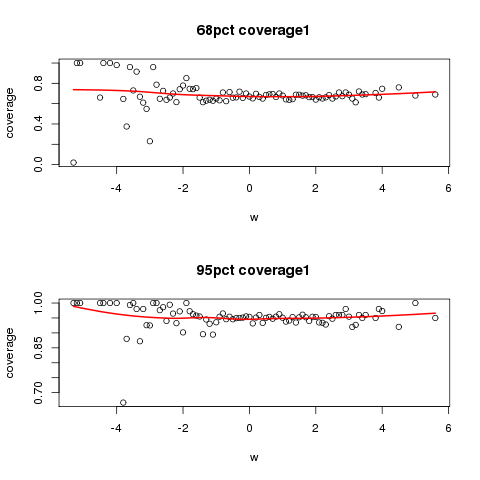
\includegraphics[width=0.5\textwidth]{YoungGentili_ps2_task4_plot1_w}
    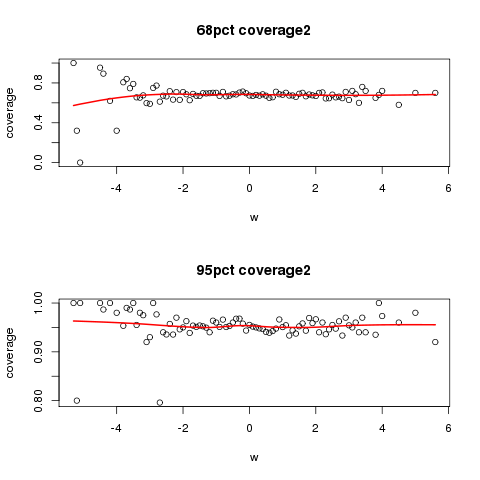
\includegraphics[width=0.5\textwidth]{YoungGentili_ps2_task4_plot2_w}
    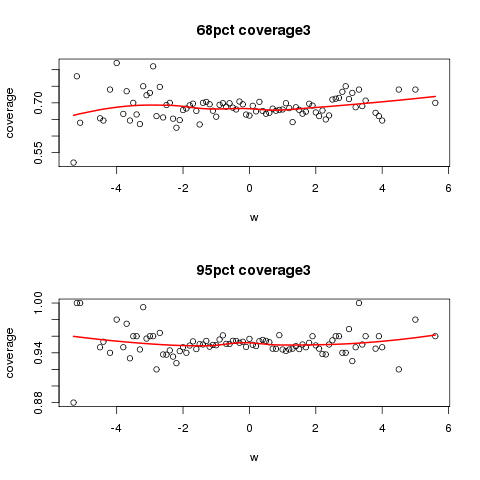
\includegraphics[width=0.5\textwidth]{YoungGentili_ps2_task4_plot3_w}
    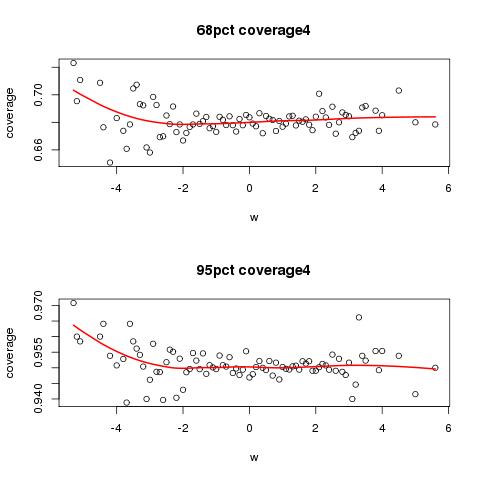
\includegraphics[width=0.5\textwidth]{YoungGentili_ps2_task4_plot4_w}
\end{figure}

\begin{figure}[h!]
  \caption{Coverage Plots for Task 4. x axis is log(theta), y-axis is coverage}

    \includegraphics[width=0.5\textwidth]{{YoungGentili_ps2_task4_plot1_logTheta.true}.png}
    \includegraphics[width=0.5\textwidth]{{YoungGentili_ps2_task4_plot2_logTheta.true}.png}
    \includegraphics[width=0.5\textwidth]{{YoungGentili_ps2_task4_plot3_logTheta.true}.png}
    \includegraphics[width=0.5\textwidth]{{YoungGentili_ps2_task4_plot4_logTheta.true}.png}
\end{figure}

\begin{figure}[h!]
  \caption{Coverage Plots for Task 5. x axis is log(w), y-axis is coverage}

    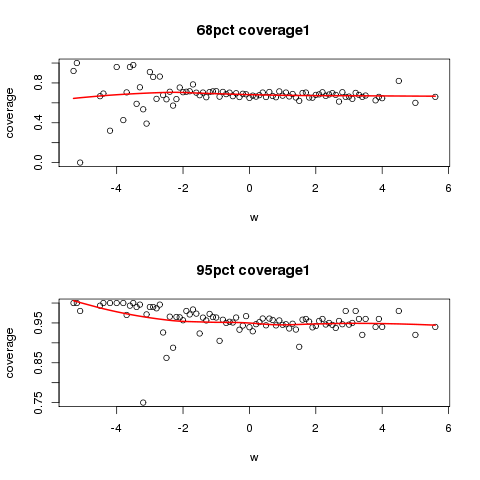
\includegraphics[width=0.5\textwidth]{YoungGentili_ps2_task5_plot1_w}
    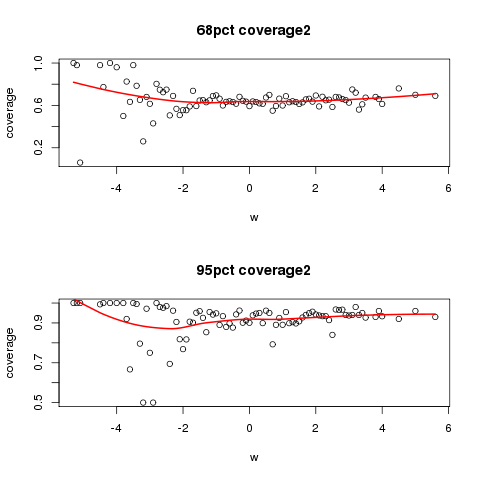
\includegraphics[width=0.5\textwidth]{YoungGentili_ps2_task5_plot2_w}
    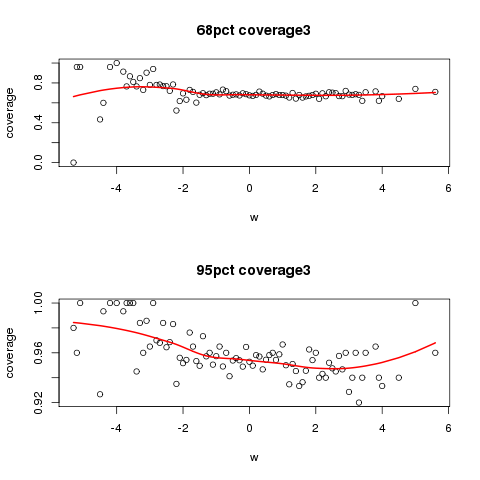
\includegraphics[width=0.5\textwidth]{YoungGentili_ps2_task5_plot3_w}
    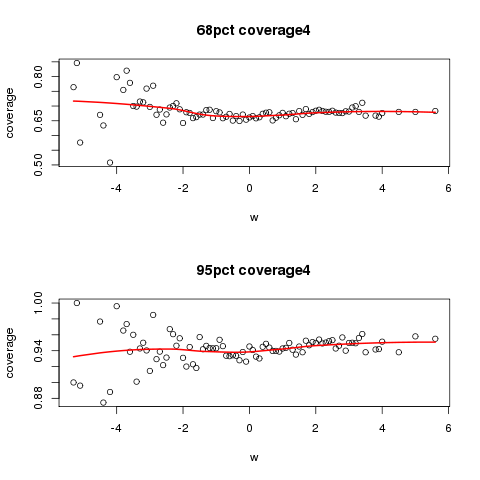
\includegraphics[width=0.5\textwidth]{YoungGentili_ps2_task5_plot4_w}
\end{figure}

\begin{figure}[h!]
  \caption{Coverage Plots for Task 5. x axis is log(theta), y-axis is coverage}

    \includegraphics[width=0.5\textwidth]{{YoungGentili_ps2_task5_plot1_logTheta.true}.png}
    \includegraphics[width=0.5\textwidth]{{YoungGentili_ps2_task5_plot2_logTheta.true}.png}
    \includegraphics[width=0.5\textwidth]{{YoungGentili_ps2_task5_plot3_logTheta.true}.png}
    \includegraphics[width=0.5\textwidth]{{YoungGentili_ps2_task5_plot4_logTheta.true}.png}
\end{figure}
\end{document}
